\section{Résultats}~\label{sec:resultats}
Un pré-traitement des données est présenté dans la~\autoref{sec:pre-traitement} afin d'évaluer la vitesse du corps du robot en filtrant le bruit.
Ensuite, les données sont utilisées pour évaluer le modèle présenté dans la~\autoref{sec:forces}.

\subsection{Pré-traitement des données}~\label{sec:pre-traitement}
En premier lieu, un traitement des données a été effectué afin d'extraire les vitesses des roues ainsi que du corps du véhicule.
Afin de respecter l'hypothèse de régime permanent et pour filtrer le bruit dans la récolte de données, la médiane de chaque valeur a été conservée pour chaque fenêtre de \SI{10}{\second}.
Suite à ce pré-traitement, le vecteur de viteses du corps du véhicule $\bm v$ et sa vitesse angulaire $\omega$ sont évalués pour chaque vitesse angulaire commandée $\omega_c$, les résultats sont montrés dans la~\autoref{fig:vitesses}.
Le vecteur $\bm v$ est mesuré à l'aide de l'algorithme \ac{ICP} et les vitesses angulaires $\omega$ sont mesurées avec la centrale inertielle.
Un modèle différentiel idéal a été utilisé pour calculer les vitesses du corps du robot en fonction des vitesses de roues. 
Ce modèle ne permet pas de modéliser la vitesse latérale du robot, ce qui explique pourquoi cette valeur demeure nulle.

\begin{figure}[htpb]
	\centering
	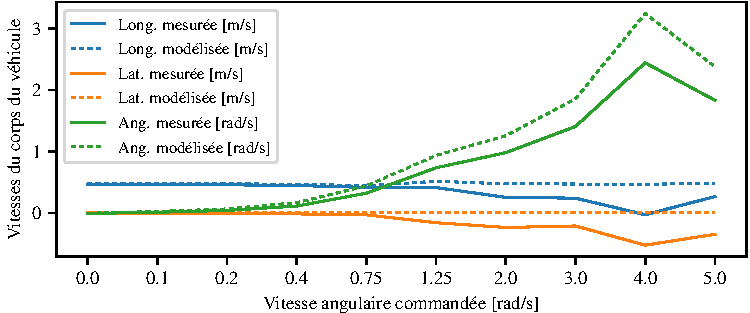
\includegraphics[width=0.48\textwidth]{figs/body_vels.pdf}
	\caption{Vitesses du corps du véhicule mesurées et modélisées dans le cadre de l'expérience en fonction de la vitesse angulaire commandée.
			La vitesse longitudinale est affichée en bleu, la vitesse latérale en orange et la vitesse angulaire en vert.
			Les vitesses mesurées avec \ac{ICP} sont montrées en lignes pleines. 
			Les vitesses estimées en fonction des vitesses des roues et d'un modèle différentiel idéal sont montrées en pointillé.}
	\label{fig:vitesses}
\end{figure}

\subsection{Évaluation des forces}~\label{sec:forces}
En premier, il est nécessaire d'évaluer les données qui servent d'entrées du modèle de force de contact. 
En fonction des vitesses du corps du robot, la position du centre de rotation instantané est calculée en suivant l'\autoref{eqn:icr}.
Ensuite, les angles de dérive de chaque roue sont évalués, ceux-ci sont montrés dans la~\autoref{fig:angles}.
Dans cette figure, les angles de dérive $\gamma_i$ sont mesurés avec \ac{ICP} et modélisés en fonction des vitesses de roues et du modèle différentiel idéal.
Il est possible d'observer qu'en fonction de l'augmentation de vitesse angulaire commandée, l'angle de dérive augmente, jusqu'à plafonner et se stabiliser. 
Le pic d'angle de dérive pour les roues 1 et 3 semble se produire légèrement après le passage du centre de rotation instantané à l'intérieur de l'empattement du \ac{VSS}.

\begin{figure}[htpb]
	\centering
	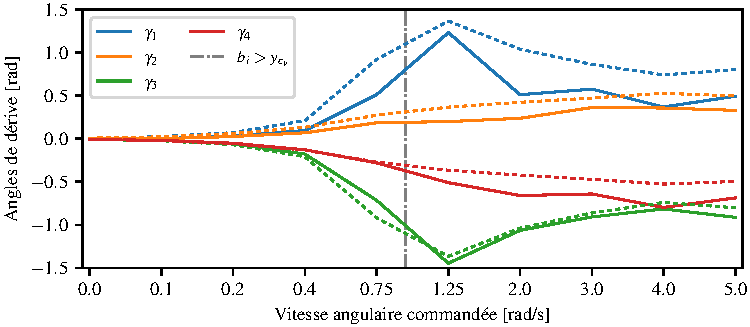
\includegraphics[width=0.48\textwidth]{figs/slip_angles.pdf}
	\caption{Angles de dérives pour chaque roue en fonction de la vitesse angulaire commandée pendant l'expérience.
			La roue 1 (en bleu) est à l'avant-gauche, la roue 2 (en orange) est à l'avant-droite, la roue 3 (en vert) est à l'arrière-gauche et la roue 4 (en rouge) est à l'arrière-droite.
			Encore une fois, les valeurs mesurées avec \ac{ICP} sont montrées avec des lignes pleines et les valeurs modélisées avec les vitesses de roues en pointillés.
			La ligne grise représente le moment où le centre de rotation instantané $\bm c_v$ se trouve entre les roues du véhicule.}
	\label{fig:angles}
\end{figure}

Ensuite, ces angles de dérive sont utilisés avec le modèle linéaire présenté dans l'\autoref{eqn:forces}.
La somme des forces latérales subies par le robot ainsi que son accélération centripète peuvent donc être calculées et l'égalité de l'\autoref{eqn:forces_sum} peut être vérifiée.
Les résultats pour les deux côtés de l'équation sont présentés dans la~\autoref{fig:acceleration}.
Afin de pouvoir calculer le modèle linéaire, une calibration manuelle a été faite pour déterminer la valeur du coefficient linéaire $\alpha_{lat}$ qui minimise l'erreur du modèle.
Ces valeurs sont similaires pour les angles de dérive (\ie~$\alpha_{lat} = 32$) ou les vitesses latérales (\ie~$\alpha_{lat} = 30$).

La force centripète est affichée en bleu et la somme des forces latérales subies par le véhicule est montrée en orange.
Comme mentionné dans la~\autoref{sec:modele}, nous avons observé que plusieurs articles dans l'état de l'art calculent les forces de contact en remplaçant l'angle de dérive par la vitesse latérale du point de contact de la roue.
La somme des forces calculées avec les vitesses latérales est affichée en vert.
Les forces ont été calculées avec les mesures d'\ac{ICP} ainsi qu'en utilisant les vitesses de roues.
Comme le modèle différentiel ne permet pas de vitesses latérales, la somme des forces latérales calculées avec les vitesses de roues est toujours nulle.

\begin{figure}[htpb]
	\centering
	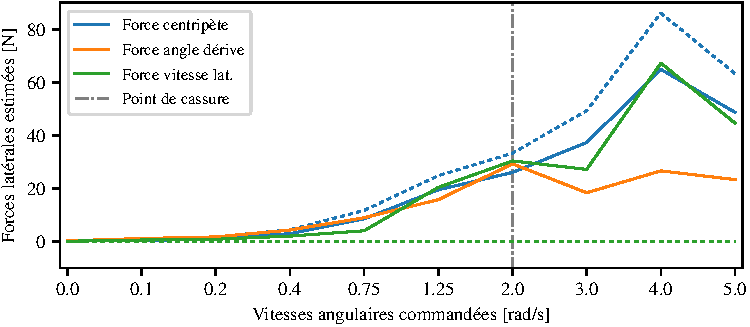
\includegraphics[width=0.48\textwidth]{figs/lateral_forces.pdf}
	\caption{Forces subies par le corps du véhicule en fonction des vitesses angulaire commandées pendant l'expérience.
			La force centripète est affichée en bleu, la somme des forces latérales calculées avec l'angle de dérive est montrée en orange et la somme des forces latérales calculées avec la vitesse latérale du point de contact est affichée en vert.
			Comme pour les figures précédentes, les valeurs mesurées avec \ac{ICP} sont montrées en lignes pleines et les forces calculées en fonction des vitesses de roues et le modèle différentiel idéal en pointillé.
			Pour les forces calculées avec un angle de dérive, il est possible d'observer un point de cassure montré avec la ligne verticale grise.}
	\label{fig:acceleration}
\end{figure}

Il est possible d'observer une faible disparité entre la force centripète et les forces calculées avec un modèle linéaire dans la~\autoref{fig:acceleration}.
De plus, il est possible d'observer un point de cassure à une vitesse angulaire commandée de \SI{2.0}{\radian\per\second}.
À cette vitesse, il est possible d'observer un pic dans la force centripète, qui peut être modélisé avec les vitesses de contact latérales, mais pas avec l'angle de dérive.
